\documentclass{pnastwo}
\usepackage{color}
\usepackage{graphicx}
\usepackage{amssymb,amsfonts,amsmath}
\usepackage{lineno}
\usepackage{multirow}
\usepackage{color}
	 \definecolor{darkred}{rgb}{0.75,0,0}
	 \definecolor{darkgreen}{rgb}{0,0.5,0}
	 \definecolor{darkblue}{rgb}{0,0,0.75}
\newcommand{\cha}[1]{\textcolor{darkblue}{#1}}
\newcommand{\arne}[1]{\textcolor{darkred}{#1}}


\usepackage[sort&compress]{}


\begin{document}

\title{Population dynamics of mutualisms}

 \author{Chaitanya S. Gokhale\affil{1}{New Zealand Institute for Advanced Study, Massey University, Auckland, New Zealand}}


\maketitle

\begin{article}

\begin{abstract}
Mutualistic relationships pose a conundrum for evolutionary theory.
Species that exploit other species would do better than sustaining a long drawn out mutually costly relationship. However we do see mutualistic relationships amongst even the most unlikely partners \ldots.
Eco-evolutionary dynamics \ldots
\end{abstract}


\keywords{mutualism | evolutionary game theory | multiple players
}

\section{Introduction}

In his book 'The History of Animals', Aristotle observes
{\em
`When the crocodile yawns, the trochilus flies into his mouth and cleans
his teeth. The trochilus gets his food thereby, and the crocodile
gets ease and comfort; it makes no attempt to injure its little friend,
but, when it wants it to go, it shakes its neck in warning, lest it
should accidentally bite the bird'} \cite{aristotle:350bc}.
The phenomenon described by Aristotle was termed as mutualism in $1873$ by the Belgian zoologist Pierre van Beneden \cite{bronstein:book:2003}.
Mutualistic relationships, interspecific interactions that benefit both species, have been empirically studied for many years 
\cite{boucher:book:1985,hinton:PTENHS:1951,wilson:AmNat:1983,bronstein:QRB:1994,pierce:ARE:2002,kiers:Nature:2003,bshary:ASB:2004} and also a considerable body of theory has been put forth trying to explain the evolution and maintenance of such relationships \cite{poulin:JTB:1995,doebeli:PNAS:1998,noe:book:2001,johnstone:ECL:2002,bergstrom:PNAS:2003,hoeksema:AmNat:2003,akcay:PRSB:2007,bshary:Nature:2008}.
The example described by Aristotle and most other examples of mutualisms lend themselves to the idea of direct reciprocity \cite{trivers:QRB:1971} and thus can be studied using evolutionary game theory.
The interactions in these models are usually dyadic.
A representative of each species is chosen and the outcome of the interactions between these representatives 
determines the evolutionary dynamics within each of the two species.
However, in many cases interactions between species cannot be reduced to such dyadic encounters \cite{stadler:book:2008}.

For example, in the interaction between ants and aphids or butterfly larvae \cite{pierce:BES:1987,hoelldobler:book:1990} many ants tend to these soft bodies creatures, providing them with shelter and protection from predation and parasites in exchange for honeydew, a rich source of food for the ants \cite{hill:OEC:1989,stadler:book:2008}.
This is not a one to one interaction between a larva and an ant, but rather a one to many interaction from the perspective of the larva.
In this manuscript we focus on this kind of -- possibly -- many to many interactions between two mutualistic species.

To analyze how benefits are shared between the two mutualistic species, we make use of evolutionary game theory.
Since we consider the interaction of two species, we resort to bimatrix games
\cite{weibull:book:1995,hofbauer:JMB:1996,hofbauer:book:1998}.



\section{Model and Results}

\subsection{Intraspecies dynamics}

Usually when interspecies relationships such as mutualism (or antagonist relationships as in predator-prey) are considered, the within species interactions are ignored for the sake of convenience. Including intraspecies interactions can however result in qualitatively different and rich dynamics which has implications for interspecies relationships.
Since we focus on mutualism the interspecies dynamics  ifs given by the multiplayer version of the snowdrift game \cite{bergstrom:PNAS:2003,souza:JTB:2009,gokhale:PRSB:2012}.
Each species consists of two types of individuals Generous $G$ and Selfish $S$. 
The details of the game are included in the Appendix, but the gist is that if everyone is Generous and contributing in the generation of mutual benefits then one can get away with being a bit selfish. All selfish is however and unstable equilibrium 

\subsection{Population dynamics}
Consider two species ($1/2$) occupying different niches in an ecosystem.
Thus we assume them to have independent carrying capacities. Each species has a normalized carrying capacity of $1$. Each species has two types the \textit{``Generous"} ones ($G_{1/2}$) who invest in a mutualistic relationship with the other species and \textit{``Selfish"} ones ($S_{1/2}$) who invest much less than their counterparts. The densities of the two types are denoted by $x_{1/2}$ and $y_{1/2}$ respectively which can sum up to the carrying capacity or not thus resulting in possible empty spaces in the niche $z_{1,2}$. Thus in all we have $x_{1/2} + y_{1/2} + z_{1/2} = 1$.
Thus how the population densities change over time $x_{1/2} + y(1/2)$ can give us a picture of the population dynamics.
\subsection{Evolutionary dynamics}
The two species are assumed to be engaged in a mutualistic relationship. This can be aptly described by a snowdrift game \cite{souza:JTB:2009}. In a general form, a number of individuals from one species interacts with a number of individuals from the other species (excluding intra species interactions) \cite{gokhale:PRSB:2012}. 
The densities of the two types of individuals in each species \textit{``Generous"} and \textit{``Selfish"} can be interpreted as probabilities of picking the two types. Thus the evolution of the fraction of one of the types, say \textit{``Generous"} over time provides us with the relevant evolutionary dynamics. The fraction of \textit{``Generous"} players is given by $f_{1/2} = x_{1/2} / (1- z_{1/2} )$.

\begin{figure}[h]
\begin{center}
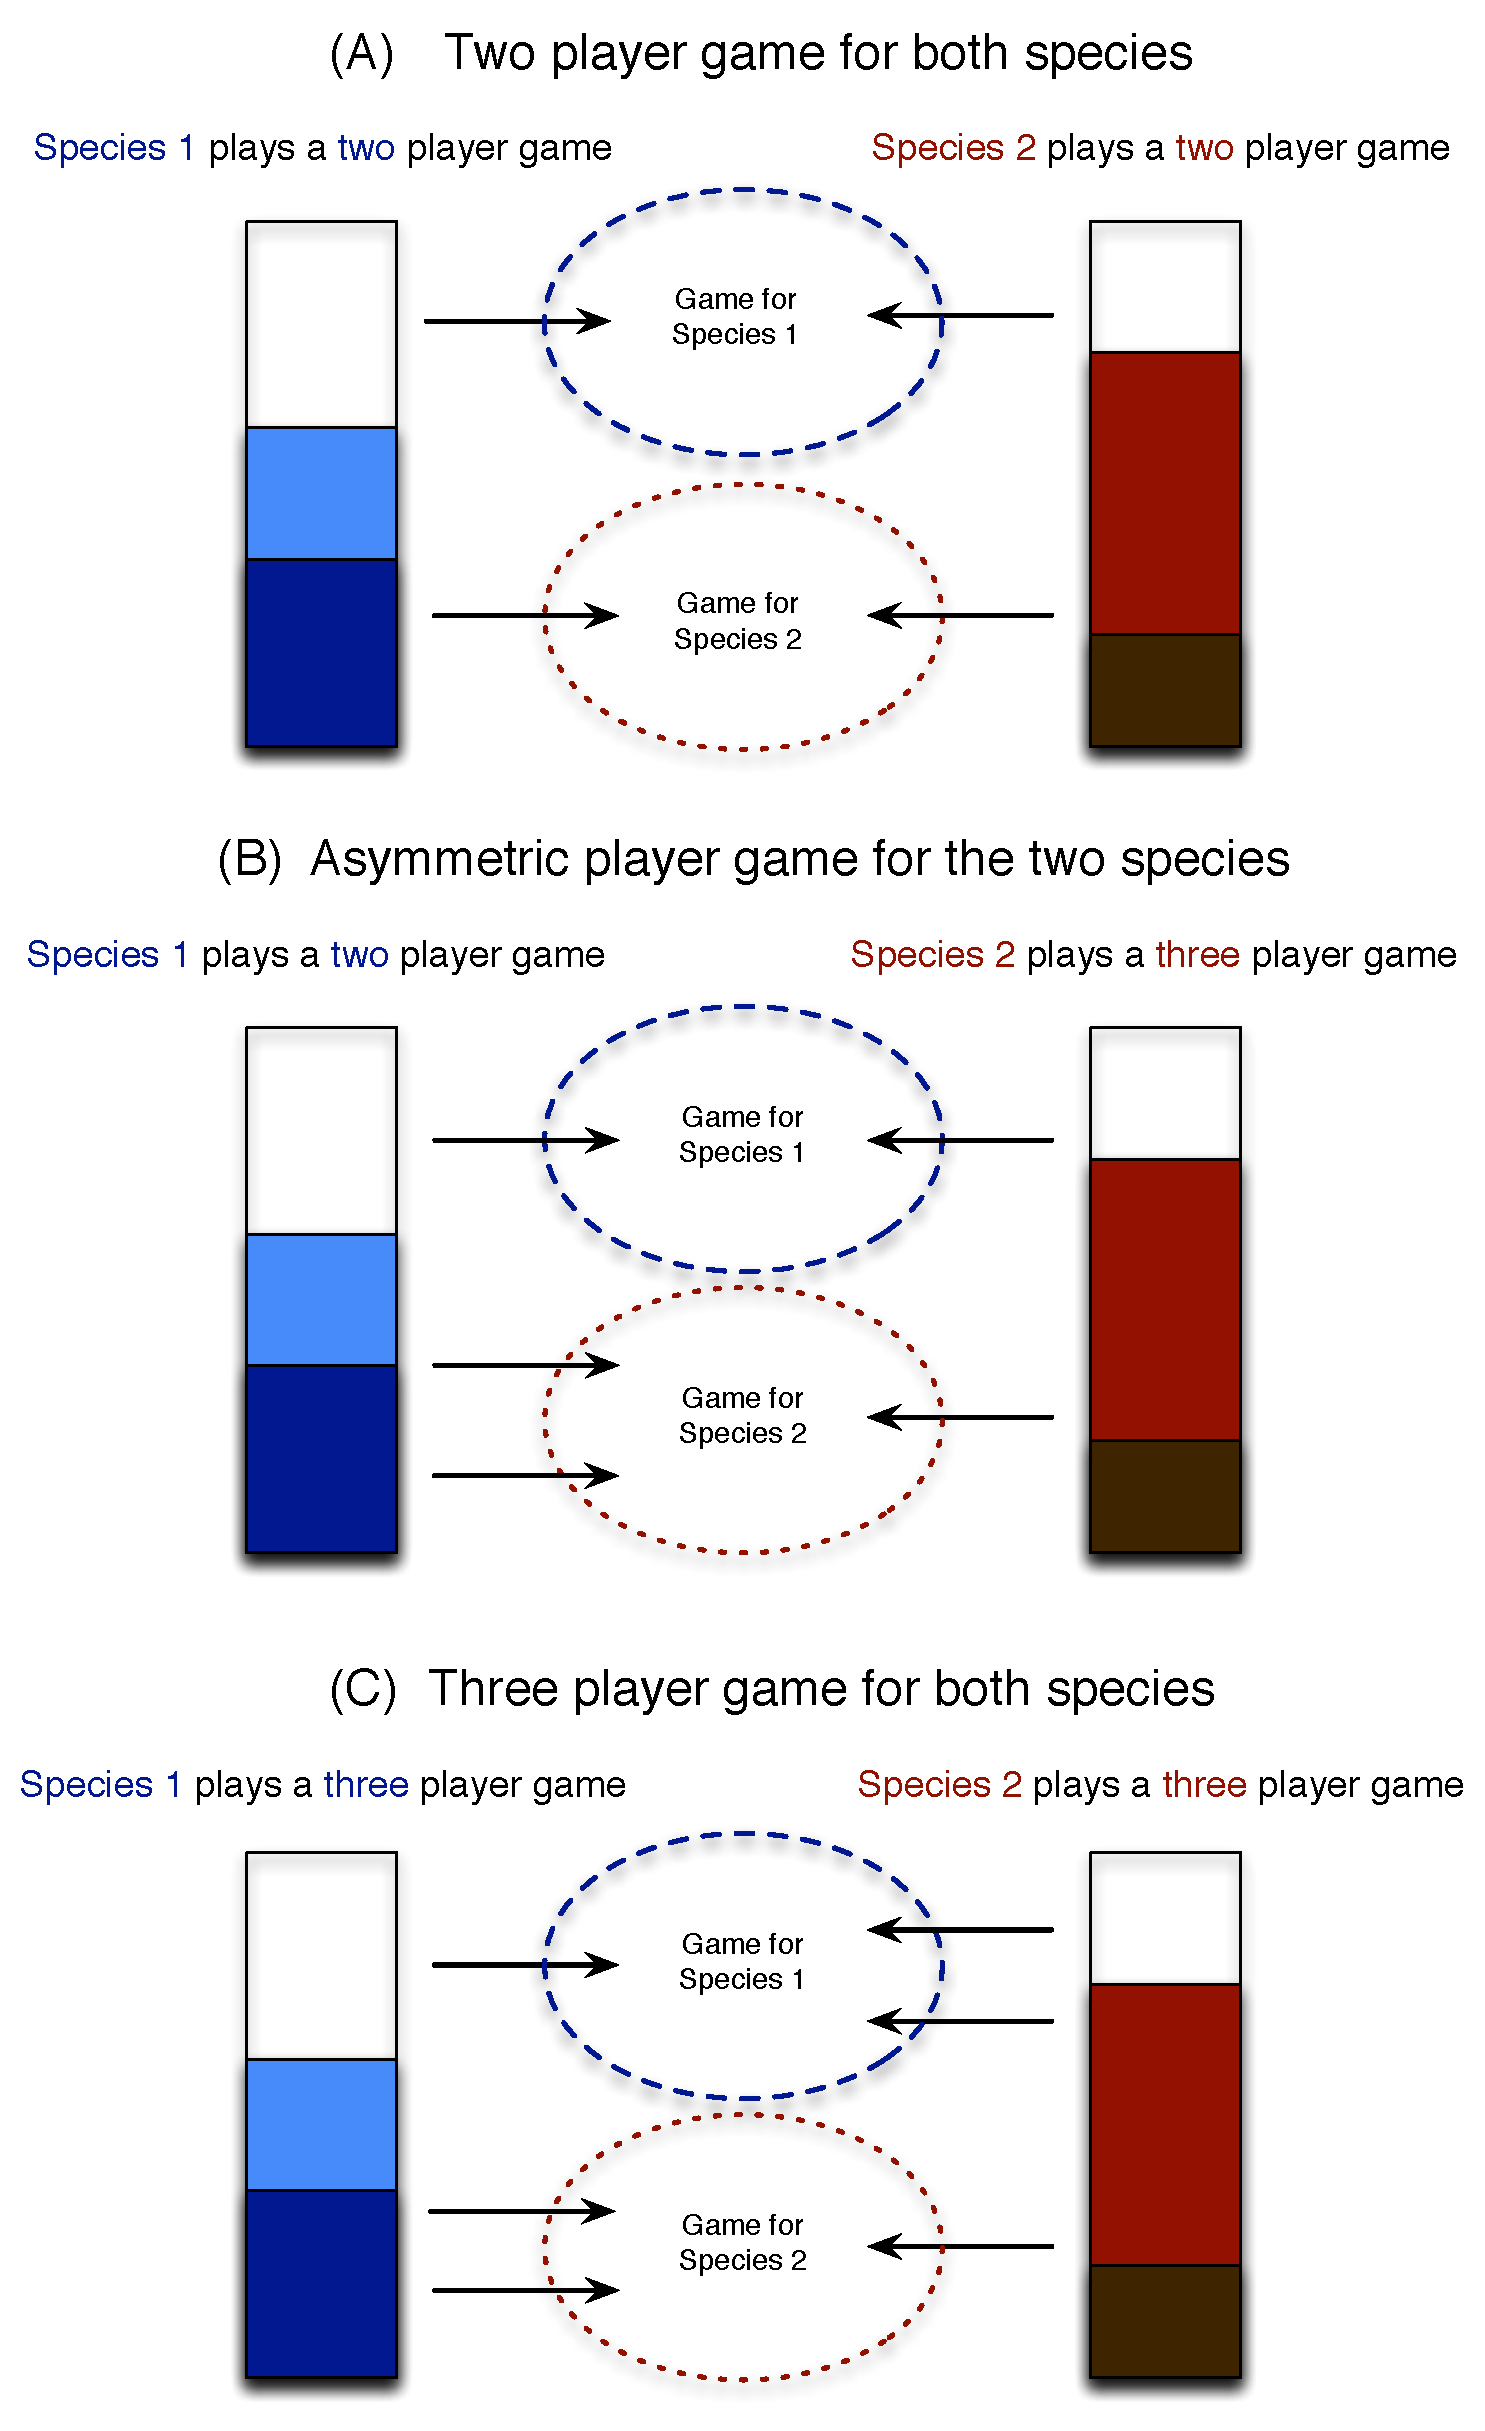
\includegraphics[width=\columnwidth]{concept.pdf}
\caption{
The composition of both species can range from all selfish $(S)$ to all generous $(G)$. 
If the other species is sufficiently generous, selfish behavior is favored in both species.
However, if the other species is selfish, generous behavior is advantageous.  
This is captured by the snowdrift game discussed in the text.
For equal evolutionary rates, $r_x=r_y$, the domains of attraction for the two outcomes $(S_1, G_2)$ and $(G_1, S_2)$
are of equal size (Panels A and C).
The colors illustrate the regions leading to the outcomes favorable to species $1$ (blue shaded area leading to $(S_1, G_2)$) 
and species $2$ (red shaded area leading to $(G_1, S_2)$).
For a two player game, $d=2$, and $r_x=r_y/8$, the basin of attraction favorable to the slower evolving species $1$ grows substantially (Panel B) \cite{bergstrom:2003jf}.
For a twenty player game, $d=20$, the basins of attractions have identical size for equal evolutionary rates, but the position of the internal equilibrium is shifted (Panel C).
When species $1$ evolves slower than species $2$ in this situation, most of the initial conditions in the simplex lead to a solution which is unfavorable to species $1$.
Thus for 20 players instead of two, the Red King effect is reversed ($b=2$ and $c=1$).
\label{fig:compare}
}
\end{center}
\end{figure}

\section{Discussion}




\begin{acknowledgments}
Thanks for all the fish
\end{acknowledgments}




\appendix

\section*{Appendix}

\section{Dynamics with single types}

Assuming that each of the species is homogeneous in terms of the kind of individuals it harbours we have a simplified system.
In species 1 we have $x$ as the density of the individuals and $z_1$ as the empty space (which is simply $1-x$).
Respectively in species 2 it is $y$ and $z_2$ (which is $1-y$).
The fitness of each of the species is then,
%
\begin{align}
f_{1} (y) &= \sum_{k=0}^{d-1} \binom{d-1}{k}y^k z_2 ^{d-1-k} \Pi(k) \\
f_{2} (x) &= \sum_{k=0}^{d-1} \binom{d-1}{k}x^k z_1 ^{d-1-k} \Pi(k).
\label{simpfiteqs}
\end{align}
%
where 
\begin{align}
\Pi (k) & = \begin{cases} b-\frac{c}{k} & \textrm{if } k \geq M \\  -\frac{c}{M} & \textrm{if } k < M 
\end{cases}	
\end{align}
The dynamics of the two species is then given by the typical Verhulst equation,

\begin{align}
	\dot{x} &= f_{1}(y) x z_1 \\
	\dot{y} &= f_{2}(x) y z_2
\end{align}

\cha{This should be easy dynamics to calculate the equilibrium, only cooperators}

\section*{Average payoffs in the bimatrix game}
\label{appA}
\subsection{Two player setting}

We can write down the payoff matrices for the two species separately  denoted by $A$ and $B$ as,
\begin{tabular}{cccccc}
& & & \multicolumn{2}{c}{Species 2} &\\
& & & $G_2$ & $S_2$ &\\
\multirow{2}{*}{$A$ = Species 1}& $G_1$
& \multirow{2}{*}{$\bigg($} & $a_{G_1,G_2}$ & $a_{G_1,S_2}$ & \multirow{2}{*}{$\bigg)$}\\
& $S_1$ & & $a_{S_1,G_2}$ & $a_{S_1,S_2}$ &
\end{tabular}
\begin{tabular}{cccccc}
& & & \multicolumn{2}{c}{Species 1} &\\
& & & $G_1$ & $S_1$ &\\
\multirow{2}{*}{B = Species 2}& $G_2$
& \multirow{2}{*}{$\bigg($} & $a_{G_2,G_1}$ & $a_{G_2,S_1}$ & \multirow{2}{*}{$\bigg)$}\\
& $S_2$ & & $a_{S_2,G_1}$ & $a_{S_2,S_1}$ &\ \ .
\end{tabular}
The frequency of the players playing strategy \textit{``Generous"} in species $1$ is given by $x$ and that in species $2$ by $y$.
As the population size is kept constant the reciprocal frequencies of the players playing \textit{``Selfish"} strategy are $1-x$ and $1-y$ in the two species respectively.

\subsection{Multiplayer setting}
\label{appB}

For a multiplayer snowdrift game, the payoff entries are defined as \cite{souza:2009aa},
\begin{align}
\Pi_{S_1} (k) & = \begin{cases} b & \textrm{if } k \geq M \\ 0 & \textrm{if } k < M \end{cases}
\\
\Pi_{G_1} (k) & = \begin{cases} b-\frac{c}{k} & \textrm{if } k \geq M \\  -\frac{c}{M} & \textrm{if } k < M \end{cases}
\end{align}
%
The selfish players get the benefit $b$ if the number of generous individuals in both species combined, $k$, is greater than or equal to the threshold $M$.
For the generous individuals, their effort is subtracted from the payoffs.
The effort is shared if the quorum size is met ($\frac{c}{M}$), but happens in vain for $k<M$. 
The fitnesses of the two strategies in species $1$ are given by,
%
\begin{align}
f_{G_1} (y) &= \sum_{k=0}^{d-1} \binom{d-1}{k}y^k (1-y)^{d-1-k} \Pi_{G_1}(k+1) \\
f_{S_1} (y) &= \sum_{k=0}^{d-1} \binom{d-1}{k}y^k (1-y)^{d-1-k} \Pi_{S_1}(k).
\label{fiteqs}
\end{align}
%
Following the same procedure for the two strategies in species $2$ leads to the average fitness
%
\begin{align}
\bar{f}_1 (x,y) &= x f_{G_1} (y)+(1-x) f_ {S_1}(y)\\
\bar{f}_2 (x,y) &= y f_{G_2} (x)+(1-y) f_{S_2}(x).
\label{avgfiteqs}
\end{align}
%

\section{Dynamics in asymmetric conditions}

We have addressed two kinds of asymmetries in the game, the number of player and the thresholds in the two species.
We denote the number of players for species $1$ and species $2$ as $d_1$ and $d_2$, respectively, as in Fig.\ \ref{fig:counter}.
That is if species $2$ is playing a $d_2$ player game it means that one player from species $2$ interacts with $d_2-1$ players of species $1$.
For an asymmetry in the thresholds we use the two parameters $M_1\geq1$ and $M_2\geq1$ for the two species, respectively.

For asymmetric bimatrix games, there is a difference in the dynamics between the standard replicator dynamics and the 
alternative dynamics put forward by Maynard-Smith \cite{maynard-smith:1982to}.
For this dynamics, the average fitness of each species appears as a denominator,
\begin{align}
\dot{x} &= r_x x \left(f_{G_1}(y) -  \bar{f}_1(x,y) \right)/\bar{f}_1(x,y) \nonumber \\
\dot{y} &= r_y y \left(f_{G_2}(x) -  \bar{f}_2(x,y) \right)/\bar{f}_2(x,y).
\label{eq:repeqs}
\end{align}
In our asymmetric bimatrix game, the fixed point stability is affected by the choice of the dynamics, in contrast to the case of symmetric games. 
In Fig.\ \ref{fig:thresholdsmodrep}, we illustrate that the dynamics is different between the usual 
replicator dynamics and Eqs. \ref{eq:repeqs}

For $d_1=d_2 \geq 5$, the exact coordinates of the fixed point must be computed numerically \cite{abel:1824aa,stewart:2004aa}.

\bibliographystyle{pnas}
\bibliography{\string~/Bibtex/et.bib}


\end{article}
\end{document}